\documentclass[1p]{elsarticle_modified}
%\bibliographystyle{elsarticle-num}

%\usepackage[colorlinks]{hyperref}
%\usepackage{abbrmath_seonhwa} %\Abb, \Ascr, \Acal ,\Abf, \Afrak
\usepackage{amsfonts}
\usepackage{amssymb}
\usepackage{amsmath}
\usepackage{amsthm}
\usepackage{scalefnt}
\usepackage{amsbsy}
\usepackage{kotex}
\usepackage{caption}
\usepackage{subfig}
\usepackage{color}
\usepackage{graphicx}
\usepackage{xcolor} %% white, black, red, green, blue, cyan, magenta, yellow
\usepackage{float}
\usepackage{setspace}
\usepackage{hyperref}

\usepackage{tikz}
\usetikzlibrary{arrows}

\usepackage{multirow}
\usepackage{array} % fixed length table
\usepackage{hhline}

%%%%%%%%%%%%%%%%%%%%%
\makeatletter
\renewcommand*\env@matrix[1][\arraystretch]{%
	\edef\arraystretch{#1}%
	\hskip -\arraycolsep
	\let\@ifnextchar\new@ifnextchar
	\array{*\c@MaxMatrixCols c}}
\makeatother %https://tex.stackexchange.com/questions/14071/how-can-i-increase-the-line-spacing-in-a-matrix
%%%%%%%%%%%%%%%

\usepackage[normalem]{ulem}

\newcommand{\msout}[1]{\ifmmode\text{\sout{\ensuremath{#1}}}\else\sout{#1}\fi}
%SOURCE: \msout is \stkout macro in https://tex.stackexchange.com/questions/20609/strikeout-in-math-mode

\newcommand{\cancel}[1]{
	\ifmmode
	{\color{red}\msout{#1}}
	\else
	{\color{red}\sout{#1}}
	\fi
}

\newcommand{\add}[1]{
	{\color{blue}\uwave{#1}}
}

\newcommand{\replace}[2]{
	\ifmmode
	{\color{red}\msout{#1}}{\color{blue}\uwave{#2}}
	\else
	{\color{red}\sout{#1}}{\color{blue}\uwave{#2}}
	\fi
}

\newcommand{\Sol}{\mathcal{S}} %segment
\newcommand{\D}{D} %diagram
\newcommand{\A}{\mathcal{A}} %arc


%%%%%%%%%%%%%%%%%%%%%%%%%%%%%5 test

\def\sl{\operatorname{\textup{SL}}(2,\Cbb)}
\def\psl{\operatorname{\textup{PSL}}(2,\Cbb)}
\def\quan{\mkern 1mu \triangleright \mkern 1mu}

\theoremstyle{definition}
\newtheorem{thm}{Theorem}[section]
\newtheorem{prop}[thm]{Proposition}
\newtheorem{lem}[thm]{Lemma}
\newtheorem{ques}[thm]{Question}
\newtheorem{cor}[thm]{Corollary}
\newtheorem{defn}[thm]{Definition}
\newtheorem{exam}[thm]{Example}
\newtheorem{rmk}[thm]{Remark}
\newtheorem{alg}[thm]{Algorithm}

\newcommand{\I}{\sqrt{-1}}
\begin{document}

%\begin{frontmatter}
%
%\title{Boundary parabolic representations of knots up to 8 crossings}
%
%%% Group authors per affiliation:
%\author{Yunhi Cho} 
%\address{Department of Mathematics, University of Seoul, Seoul, Korea}
%\ead{yhcho@uos.ac.kr}
%
%
%\author{Seonhwa Kim} %\fnref{s_kim}}
%\address{Center for Geometry and Physics, Institute for Basic Science, Pohang, 37673, Korea}
%\ead{ryeona17@ibs.re.kr}
%
%\author{Hyuk Kim}
%\address{Department of Mathematical Sciences, Seoul National University, Seoul 08826, Korea}
%\ead{hyukkim@snu.ac.kr}
%
%\author{Seokbeom Yoon}
%\address{Department of Mathematical Sciences, Seoul National University, Seoul, 08826,  Korea}
%\ead{sbyoon15@snu.ac.kr}
%
%\begin{abstract}
%We find all boundary parabolic representation of knots up to 8 crossings.
%
%\end{abstract}
%\begin{keyword}
%    \MSC[2010] 57M25 
%\end{keyword}
%
%\end{frontmatter}

%\linenumbers
%\tableofcontents
%
\newcommand\colored[1]{\textcolor{white}{\rule[-0.35ex]{0.8em}{1.4ex}}\kern-0.8em\color{red} #1}%
%\newcommand\colored[1]{\textcolor{white}{ #1}\kern-2.17ex	\textcolor{white}{ #1}\kern-1.81ex	\textcolor{white}{ #1}\kern-2.15ex\color{red}#1	}

{\Large $\underline{12a_{0508}~(K12a_{0508})}$}

\setlength{\tabcolsep}{10pt}
\renewcommand{\arraystretch}{1.6}
\vspace{1cm}\begin{tabular}{m{100pt}>{\centering\arraybackslash}m{274pt}}
\multirow{5}{120pt}{
	\centering
	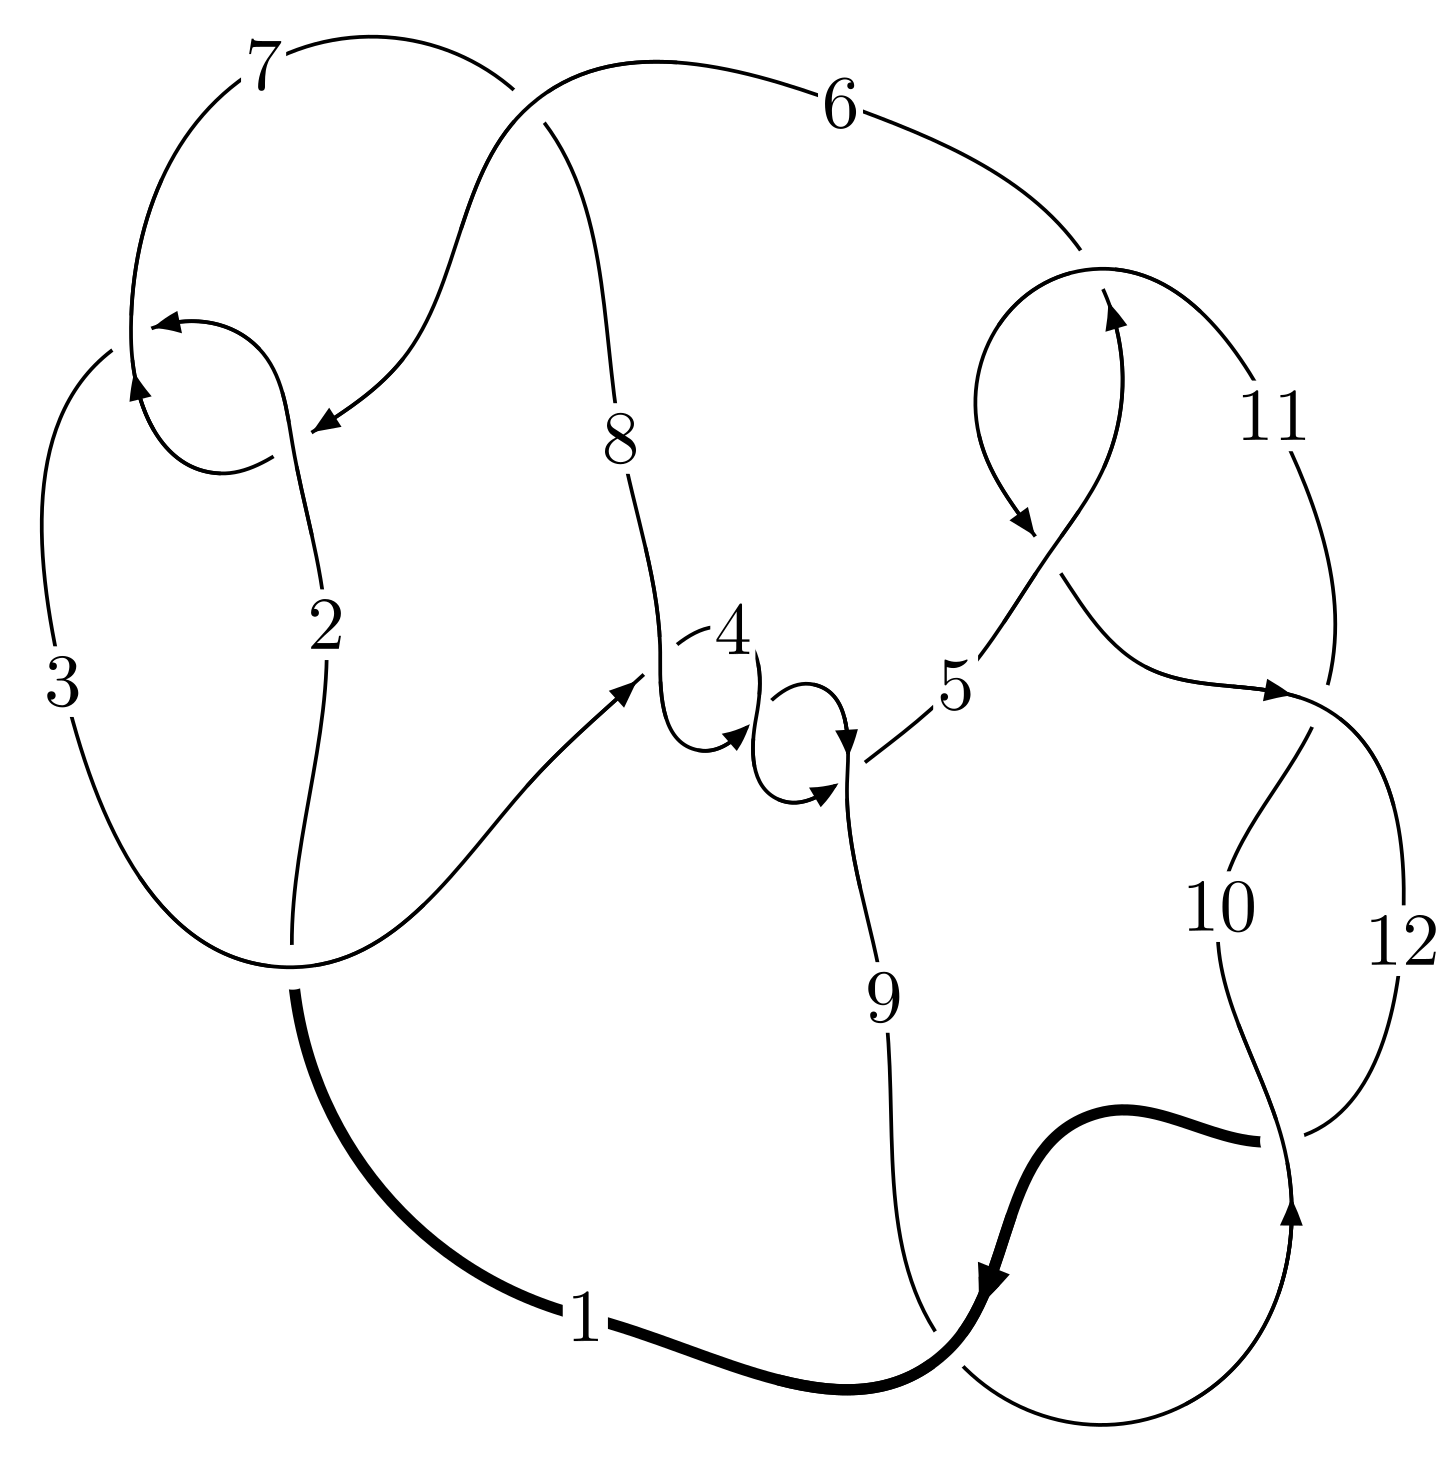
\includegraphics[width=112pt]{../../../GIT/diagram.site/Diagrams/png/1309_12a_0508.png}\\
\ \ \ A knot diagram\footnotemark}&
\allowdisplaybreaks
\textbf{Linearized knot diagam} \\
\cline{2-2}
 &
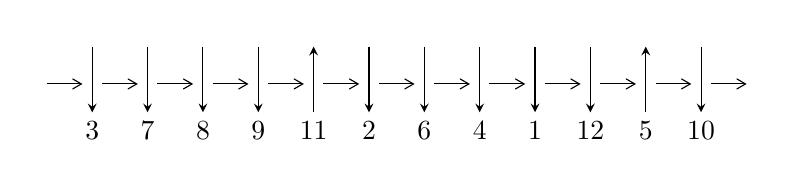
\begin{tikzpicture}[x=20pt, y=17pt]
	% nodes
	\node (C0) at (0, 0) {};
	\node (C1) at (1, 0) {};
	\node (C1U) at (1, +1) {};
	\node (C1D) at (1, -1) {3};

	\node (C2) at (2, 0) {};
	\node (C2U) at (2, +1) {};
	\node (C2D) at (2, -1) {7};

	\node (C3) at (3, 0) {};
	\node (C3U) at (3, +1) {};
	\node (C3D) at (3, -1) {8};

	\node (C4) at (4, 0) {};
	\node (C4U) at (4, +1) {};
	\node (C4D) at (4, -1) {9};

	\node (C5) at (5, 0) {};
	\node (C5U) at (5, +1) {};
	\node (C5D) at (5, -1) {11};

	\node (C6) at (6, 0) {};
	\node (C6U) at (6, +1) {};
	\node (C6D) at (6, -1) {2};

	\node (C7) at (7, 0) {};
	\node (C7U) at (7, +1) {};
	\node (C7D) at (7, -1) {6};

	\node (C8) at (8, 0) {};
	\node (C8U) at (8, +1) {};
	\node (C8D) at (8, -1) {4};

	\node (C9) at (9, 0) {};
	\node (C9U) at (9, +1) {};
	\node (C9D) at (9, -1) {1};

	\node (C10) at (10, 0) {};
	\node (C10U) at (10, +1) {};
	\node (C10D) at (10, -1) {12};

	\node (C11) at (11, 0) {};
	\node (C11U) at (11, +1) {};
	\node (C11D) at (11, -1) {5};

	\node (C12) at (12, 0) {};
	\node (C12U) at (12, +1) {};
	\node (C12D) at (12, -1) {10};
	\node (C13) at (13, 0) {};

	% arrows
	\draw[->,>={angle 60}]
	(C0) edge (C1) (C1) edge (C2) (C2) edge (C3) (C3) edge (C4) (C4) edge (C5) (C5) edge (C6) (C6) edge (C7) (C7) edge (C8) (C8) edge (C9) (C9) edge (C10) (C10) edge (C11) (C11) edge (C12) (C12) edge (C13) ;	\draw[->,>=stealth]
	(C1U) edge (C1D) (C2U) edge (C2D) (C3U) edge (C3D) (C4U) edge (C4D) (C5D) edge (C5U) (C6U) edge (C6D) (C7U) edge (C7D) (C8U) edge (C8D) (C9U) edge (C9D) (C10U) edge (C10D) (C11D) edge (C11U) (C12U) edge (C12D) ;
	\end{tikzpicture} \\
\hhline{~~} \\& 
\textbf{Solving Sequence} \\ \cline{2-2} 
 &
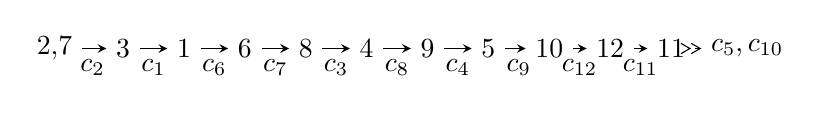
\begin{tikzpicture}[x=22pt, y=7pt]
	% node
	\node (A0) at (-1/8, 0) {2,7};
	\node (A1) at (1, 0) {3};
	\node (A2) at (2, 0) {1};
	\node (A3) at (3, 0) {6};
	\node (A4) at (4, 0) {8};
	\node (A5) at (5, 0) {4};
	\node (A6) at (6, 0) {9};
	\node (A7) at (7, 0) {5};
	\node (A8) at (8, 0) {10};
	\node (A9) at (9, 0) {12};
	\node (A10) at (10, 0) {11};
	\node (C1) at (1/2, -1) {$c_{2}$};
	\node (C2) at (3/2, -1) {$c_{1}$};
	\node (C3) at (5/2, -1) {$c_{6}$};
	\node (C4) at (7/2, -1) {$c_{7}$};
	\node (C5) at (9/2, -1) {$c_{3}$};
	\node (C6) at (11/2, -1) {$c_{8}$};
	\node (C7) at (13/2, -1) {$c_{4}$};
	\node (C8) at (15/2, -1) {$c_{9}$};
	\node (C9) at (17/2, -1) {$c_{12}$};
	\node (C10) at (19/2, -1) {$c_{11}$};
	\node (A11) at (45/4, 0) {$c_{5},c_{10}$};

	% edge
	\draw[->,>=stealth]	
	(A0) edge (A1) (A1) edge (A2) (A2) edge (A3) (A3) edge (A4) (A4) edge (A5) (A5) edge (A6) (A6) edge (A7) (A7) edge (A8) (A8) edge (A9) (A9) edge (A10) ;
	\draw[->>,>={angle 60}]	
	(A10) edge (A11);
\end{tikzpicture} \\ 

\end{tabular} \\

\footnotetext{
The image of knot diagram is generated by the software ``\textbf{Draw programme}" developed by Andrew Bartholomew(\url{http://www.layer8.co.uk/maths/draw/index.htm\#Running-draw}), where we modified some parts for our purpose(\url{https://github.com/CATsTAILs/LinksPainter}).
}\phantom \\ \newline 
\centering \textbf{Ideals for irreducible components\footnotemark of $X_{\text{par}}$} 
 
\begin{align*}
I^u_{1}&=\langle 
u^{64}- u^{63}+\cdots-2 u-1\rangle \\
\\
\end{align*}
\raggedright * 1 irreducible components of $\dim_{\mathbb{C}}=0$, with total 64 representations.\\
\footnotetext{All coefficients of polynomials are rational numbers. But the coefficients are sometimes approximated in decimal forms when there is not enough margin.}
\newpage
\renewcommand{\arraystretch}{1}
\centering \section*{I. $I^u_{1}= \langle u^{64}- u^{63}+\cdots-2 u-1 \rangle$}
\flushleft \textbf{(i) Arc colorings}\\
\begin{tabular}{m{7pt} m{180pt} m{7pt} m{180pt} }
\flushright $a_{2}=$&$\begin{pmatrix}1\\0\end{pmatrix}$ \\
\flushright $a_{7}=$&$\begin{pmatrix}0\\u\end{pmatrix}$ \\
\flushright $a_{3}=$&$\begin{pmatrix}1\\u^2\end{pmatrix}$ \\
\flushright $a_{1}=$&$\begin{pmatrix}- u^2+1\\- u^4\end{pmatrix}$ \\
\flushright $a_{6}=$&$\begin{pmatrix}u\\u\end{pmatrix}$ \\
\flushright $a_{8}=$&$\begin{pmatrix}- u^3\\- u^3+u\end{pmatrix}$ \\
\flushright $a_{4}=$&$\begin{pmatrix}- u^8+u^6- u^4+1\\- u^8+2 u^6-2 u^4+2 u^2\end{pmatrix}$ \\
\flushright $a_{9}=$&$\begin{pmatrix}u^{13}-2 u^{11}+3 u^9-2 u^7- u\\u^{13}-3 u^{11}+5 u^9-6 u^7+4 u^5-3 u^3+u\end{pmatrix}$ \\
\flushright $a_{5}=$&$\begin{pmatrix}u^{18}-3 u^{16}+6 u^{14}-7 u^{12}+5 u^{10}-3 u^8- u^2+1\\u^{18}-4 u^{16}+9 u^{14}-14 u^{12}+15 u^{10}-14 u^8+10 u^6-6 u^4+3 u^2\end{pmatrix}$ \\
\flushright $a_{10}=$&$\begin{pmatrix}u^{19}-4 u^{17}+10 u^{15}-16 u^{13}+19 u^{11}-18 u^9+14 u^7-10 u^5+5 u^3-2 u\\u^{21}-3 u^{19}+\cdots-3 u^3+u\end{pmatrix}$ \\
\flushright $a_{12}=$&$\begin{pmatrix}- u^{36}+7 u^{34}+\cdots+u^2+1\\- u^{38}+6 u^{36}+\cdots+6 u^4- u^2\end{pmatrix}$ \\
\flushright $a_{11}=$&$\begin{pmatrix}u^{53}-10 u^{51}+\cdots+8 u^3-3 u\\u^{55}-9 u^{53}+\cdots-2 u^3+u\end{pmatrix}$\\&\end{tabular}
\flushleft \textbf{(ii) Obstruction class $= -1$}\\~\\
\flushleft \textbf{(iii) Cusp Shapes $= -4 u^{62}+44 u^{60}+\cdots-24 u-14$}\\~\\
\newpage\renewcommand{\arraystretch}{1}
\flushleft \textbf{(iv) u-Polynomials at the component}\newline \\
\begin{tabular}{m{50pt}|m{274pt}}
Crossings & \hspace{64pt}u-Polynomials at each crossing \\
\hline $$\begin{aligned}c_{1},c_{7}\end{aligned}$$&$\begin{aligned}
&u^{64}+23 u^{63}+\cdots+20 u^2+1
\end{aligned}$\\
\hline $$\begin{aligned}c_{2},c_{6}\end{aligned}$$&$\begin{aligned}
&u^{64}- u^{63}+\cdots-2 u-1
\end{aligned}$\\
\hline $$\begin{aligned}c_{3},c_{4},c_{8}\end{aligned}$$&$\begin{aligned}
&u^{64}+u^{63}+\cdots+10 u^2-25
\end{aligned}$\\
\hline $$\begin{aligned}c_{5},c_{11}\end{aligned}$$&$\begin{aligned}
&u^{64}+u^{63}+\cdots-2 u-1
\end{aligned}$\\
\hline $$\begin{aligned}c_{9},c_{10},c_{12}\end{aligned}$$&$\begin{aligned}
&u^{64}+17 u^{63}+\cdots-20 u^2+1
\end{aligned}$\\
\hline
\end{tabular}\\~\\
\newpage\renewcommand{\arraystretch}{1}
\flushleft \textbf{(v) Riley Polynomials at the component}\newline \\
\begin{tabular}{m{50pt}|m{274pt}}
Crossings & \hspace{64pt}Riley Polynomials at each crossing \\
\hline $$\begin{aligned}c_{1},c_{7}\end{aligned}$$&$\begin{aligned}
&y^{64}+37 y^{63}+\cdots+40 y+1
\end{aligned}$\\
\hline $$\begin{aligned}c_{2},c_{6}\end{aligned}$$&$\begin{aligned}
&y^{64}-23 y^{63}+\cdots+20 y^2+1
\end{aligned}$\\
\hline $$\begin{aligned}c_{3},c_{4},c_{8}\end{aligned}$$&$\begin{aligned}
&y^{64}-59 y^{63}+\cdots-500 y+625
\end{aligned}$\\
\hline $$\begin{aligned}c_{5},c_{11}\end{aligned}$$&$\begin{aligned}
&y^{64}+17 y^{63}+\cdots-20 y^2+1
\end{aligned}$\\
\hline $$\begin{aligned}c_{9},c_{10},c_{12}\end{aligned}$$&$\begin{aligned}
&y^{64}+61 y^{63}+\cdots-40 y+1
\end{aligned}$\\
\hline
\end{tabular}\\~\\
\newpage\flushleft \textbf{(vi) Complex Volumes and Cusp Shapes}
$$\begin{array}{c|c|c}  
\text{Solutions to }I^u_{1}& \I (\text{vol} + \sqrt{-1}CS) & \text{Cusp shape}\\
 \hline 
\begin{aligned}
u &= -0.734158 + 0.668101 I\end{aligned}
 & \phantom{-}1.43109 - 1.27456 I & -5.99922 + 4.38526 I \\ \hline\begin{aligned}
u &= -0.734158 - 0.668101 I\end{aligned}
 & \phantom{-}1.43109 + 1.27456 I & -5.99922 - 4.38526 I \\ \hline\begin{aligned}
u &= \phantom{-}0.577379 + 0.799136 I\end{aligned}
 & \phantom{-}2.16758 + 9.15664 I & -5.96705 - 5.25155 I \\ \hline\begin{aligned}
u &= \phantom{-}0.577379 - 0.799136 I\end{aligned}
 & \phantom{-}2.16758 - 9.15664 I & -5.96705 + 5.25155 I \\ \hline\begin{aligned}
u &= -0.583021 + 0.792165 I\end{aligned}
 & \phantom{-}2.76820 - 3.03900 I & -4.88415 + 0.40129 I \\ \hline\begin{aligned}
u &= -0.583021 - 0.792165 I\end{aligned}
 & \phantom{-}2.76820 + 3.03900 I & -4.88415 - 0.40129 I \\ \hline\begin{aligned}
u &= \phantom{-}0.548606 + 0.780128 I\end{aligned}
 & -4.67791 + 4.46553 I & -11.24364 - 4.14724 I \\ \hline\begin{aligned}
u &= \phantom{-}0.548606 - 0.780128 I\end{aligned}
 & -4.67791 - 4.46553 I & -11.24364 + 4.14724 I \\ \hline\begin{aligned}
u &= -0.880732 + 0.573012 I\end{aligned}
 & -1.06214 + 2.24840 I & -14.4188 - 2.9053 I \\ \hline\begin{aligned}
u &= -0.880732 - 0.573012 I\end{aligned}
 & -1.06214 - 2.24840 I & -14.4188 + 2.9053 I \\ \hline\begin{aligned}
u &= \phantom{-}0.908597 + 0.273784 I\end{aligned}
 & \phantom{-}2.57323 - 5.53278 I & -10.06397 + 6.98986 I \\ \hline\begin{aligned}
u &= \phantom{-}0.908597 - 0.273784 I\end{aligned}
 & \phantom{-}2.57323 + 5.53278 I & -10.06397 - 6.98986 I \\ \hline\begin{aligned}
u &= \phantom{-}0.814938 + 0.667976 I\end{aligned}
 & \phantom{-}2.49514 - 2.06773 I & \phantom{-0.000000 -}0. + 3.71877 I \\ \hline\begin{aligned}
u &= \phantom{-}0.814938 - 0.667976 I\end{aligned}
 & \phantom{-}2.49514 + 2.06773 I & \phantom{-0.000000 } 0. - 3.71877 I \\ \hline\begin{aligned}
u &= -0.887915 + 0.310649 I\end{aligned}
 & \phantom{-}2.77545 - 0.35472 I & -9.35777 - 1.48918 I \\ \hline\begin{aligned}
u &= -0.887915 - 0.310649 I\end{aligned}
 & \phantom{-}2.77545 + 0.35472 I & -9.35777 + 1.48918 I \\ \hline\begin{aligned}
u &= -0.551226 + 0.748282 I\end{aligned}
 & -1.69458 - 1.28164 I & -5.29966 + 0.30789 I \\ \hline\begin{aligned}
u &= -0.551226 - 0.748282 I\end{aligned}
 & -1.69458 + 1.28164 I & -5.29966 - 0.30789 I \\ \hline\begin{aligned}
u &= -0.770088 + 0.744037 I\end{aligned}
 & \phantom{-}8.45315 - 3.75871 I & \phantom{-0.000000 -}0. + 2.83567 I \\ \hline\begin{aligned}
u &= -0.770088 - 0.744037 I\end{aligned}
 & \phantom{-}8.45315 + 3.75871 I & \phantom{-0.000000 } 0. - 2.83567 I \\ \hline\begin{aligned}
u &= \phantom{-}0.781202 + 0.741537 I\end{aligned}
 & \phantom{-}8.62407 - 2.42872 I & \phantom{-0.000000 } 0 \\ \hline\begin{aligned}
u &= \phantom{-}0.781202 - 0.741537 I\end{aligned}
 & \phantom{-}8.62407 + 2.42872 I & \phantom{-0.000000 } 0 \\ \hline\begin{aligned}
u &= \phantom{-}0.512976 + 0.755043 I\end{aligned}
 & -4.91649 - 1.59221 I & -11.90786 + 3.54404 I \\ \hline\begin{aligned}
u &= \phantom{-}0.512976 - 0.755043 I\end{aligned}
 & -4.91649 + 1.59221 I & -11.90786 - 3.54404 I \\ \hline\begin{aligned}
u &= \phantom{-}0.886320 + 0.663470 I\end{aligned}
 & \phantom{-}2.27623 - 3.08946 I & \phantom{-0.000000 } 0 \\ \hline\begin{aligned}
u &= \phantom{-}0.886320 - 0.663470 I\end{aligned}
 & \phantom{-}2.27623 + 3.08946 I & \phantom{-0.000000 } 0 \\ \hline\begin{aligned}
u &= \phantom{-}1.11340\phantom{ +0.000000I}\end{aligned}
 & -7.26377\phantom{ +0.000000I} & -11.6170\phantom{ +0.000000I} \\ \hline\begin{aligned}
u &= \phantom{-}1.117230 + 0.039150 I\end{aligned}
 & -3.19336 - 1.95587 I & -8.00000 + 0. I\phantom{ +0.000000I} \\ \hline\begin{aligned}
u &= \phantom{-}1.117230 - 0.039150 I\end{aligned}
 & -3.19336 + 1.95587 I & -8.00000 + 0. I\phantom{ +0.000000I} \\ \hline\begin{aligned}
u &= \phantom{-}0.869584 + 0.106333 I\end{aligned}
 & -3.24427 - 2.18605 I & -17.0727 + 6.0888 I\\
 \hline 
 \end{array}$$\newpage$$\begin{array}{c|c|c}  
\text{Solutions to }I^u_{1}& \I (\text{vol} + \sqrt{-1}CS) & \text{Cusp shape}\\
 \hline 
\begin{aligned}
u &= \phantom{-}0.869584 - 0.106333 I\end{aligned}
 & -3.24427 + 2.18605 I & -17.0727 - 6.0888 I \\ \hline\begin{aligned}
u &= -1.125770 + 0.039610 I\end{aligned}
 & -3.84567 + 8.00446 I & \phantom{-0.000000 } 0 \\ \hline\begin{aligned}
u &= -1.125770 - 0.039610 I\end{aligned}
 & -3.84567 - 8.00446 I & \phantom{-0.000000 } 0 \\ \hline\begin{aligned}
u &= -1.128630 + 0.012921 I\end{aligned}
 & -10.47200 + 3.12169 I & \phantom{-0.000000 } 0 \\ \hline\begin{aligned}
u &= -1.128630 - 0.012921 I\end{aligned}
 & -10.47200 - 3.12169 I & \phantom{-0.000000 } 0 \\ \hline\begin{aligned}
u &= \phantom{-}0.461327 + 0.727213 I\end{aligned}
 & \phantom{-}1.44734 - 6.27170 I & -6.61668 + 5.37317 I \\ \hline\begin{aligned}
u &= \phantom{-}0.461327 - 0.727213 I\end{aligned}
 & \phantom{-}1.44734 + 6.27170 I & -6.61668 - 5.37317 I \\ \hline\begin{aligned}
u &= -0.936943 + 0.658530 I\end{aligned}
 & \phantom{-}0.82334 + 6.42603 I & \phantom{-0.000000 } 0 \\ \hline\begin{aligned}
u &= -0.936943 - 0.658530 I\end{aligned}
 & \phantom{-}0.82334 - 6.42603 I & \phantom{-0.000000 } 0 \\ \hline\begin{aligned}
u &= -0.465307 + 0.705263 I\end{aligned}
 & \phantom{-}2.01780 + 0.29717 I & -5.58354 - 0.33676 I \\ \hline\begin{aligned}
u &= -0.465307 - 0.705263 I\end{aligned}
 & \phantom{-}2.01780 - 0.29717 I & -5.58354 + 0.33676 I \\ \hline\begin{aligned}
u &= \phantom{-}0.925319 + 0.713366 I\end{aligned}
 & \phantom{-}8.18783 - 3.10258 I & \phantom{-0.000000 } 0 \\ \hline\begin{aligned}
u &= \phantom{-}0.925319 - 0.713366 I\end{aligned}
 & \phantom{-}8.18783 + 3.10258 I & \phantom{-0.000000 } 0 \\ \hline\begin{aligned}
u &= -0.933860 + 0.711939 I\end{aligned}
 & \phantom{-}7.95805 + 9.29310 I & \phantom{-0.000000 } 0 \\ \hline\begin{aligned}
u &= -0.933860 - 0.711939 I\end{aligned}
 & \phantom{-}7.95805 - 9.29310 I & \phantom{-0.000000 } 0 \\ \hline\begin{aligned}
u &= -1.038150 + 0.620576 I\end{aligned}
 & \phantom{-}0.43349 + 4.75751 I & \phantom{-0.000000 } 0 \\ \hline\begin{aligned}
u &= -1.038150 - 0.620576 I\end{aligned}
 & \phantom{-}0.43349 - 4.75751 I & \phantom{-0.000000 } 0 \\ \hline\begin{aligned}
u &= \phantom{-}1.047470 + 0.619918 I\end{aligned}
 & -0.204610 + 1.166380 I & \phantom{-0.000000 } 0 \\ \hline\begin{aligned}
u &= \phantom{-}1.047470 - 0.619918 I\end{aligned}
 & -0.204610 - 1.166380 I & \phantom{-0.000000 } 0 \\ \hline\begin{aligned}
u &= -1.041800 + 0.654112 I\end{aligned}
 & -3.12169 + 6.62412 I & \phantom{-0.000000 } 0 \\ \hline\begin{aligned}
u &= -1.041800 - 0.654112 I\end{aligned}
 & -3.12169 - 6.62412 I & \phantom{-0.000000 } 0 \\ \hline\begin{aligned}
u &= \phantom{-}1.051460 + 0.642911 I\end{aligned}
 & -6.47434 - 3.70666 I & \phantom{-0.000000 } 0 \\ \hline\begin{aligned}
u &= \phantom{-}1.051460 - 0.642911 I\end{aligned}
 & -6.47434 + 3.70666 I & \phantom{-0.000000 } 0 \\ \hline\begin{aligned}
u &= \phantom{-}1.052550 + 0.660953 I\end{aligned}
 & -6.16225 - 9.90913 I & \phantom{-0.000000 } 0 \\ \hline\begin{aligned}
u &= \phantom{-}1.052550 - 0.660953 I\end{aligned}
 & -6.16225 + 9.90913 I & \phantom{-0.000000 } 0 \\ \hline\begin{aligned}
u &= -1.046730 + 0.676138 I\end{aligned}
 & \phantom{-}1.38825 + 8.57764 I & \phantom{-0.000000 } 0 \\ \hline\begin{aligned}
u &= -1.046730 - 0.676138 I\end{aligned}
 & \phantom{-}1.38825 - 8.57764 I & \phantom{-0.000000 } 0 \\ \hline\begin{aligned}
u &= \phantom{-}1.050950 + 0.676533 I\end{aligned}
 & \phantom{-}0.7567 - 14.7133 I & \phantom{-0.000000 } 0 \\ \hline\begin{aligned}
u &= \phantom{-}1.050950 - 0.676533 I\end{aligned}
 & \phantom{-}0.7567 + 14.7133 I & \phantom{-0.000000 } 0 \\ \hline\begin{aligned}
u &= -0.684394\phantom{ +0.000000I}\end{aligned}
 & -1.02359\phantom{ +0.000000I} & -9.41090\phantom{ +0.000000I}\\
 \hline 
 \end{array}$$\newpage$$\begin{array}{c|c|c}  
\text{Solutions to }I^u_{1}& \I (\text{vol} + \sqrt{-1}CS) & \text{Cusp shape}\\
 \hline 
\begin{aligned}
u &= -0.017794 + 0.518720 I\end{aligned}
 & \phantom{-}5.24287 + 3.00974 I & -2.07163 - 2.91236 I \\ \hline\begin{aligned}
u &= -0.017794 - 0.518720 I\end{aligned}
 & \phantom{-}5.24287 - 3.00974 I & -2.07163 + 2.91236 I \\ \hline\begin{aligned}
u &= -0.178281 + 0.318594 I\end{aligned}
 & -0.382136 + 0.981633 I & -6.53805 - 6.72584 I \\ \hline\begin{aligned}
u &= -0.178281 - 0.318594 I\end{aligned}
 & -0.382136 - 0.981633 I & -6.53805 + 6.72584 I\\
 \hline 
 \end{array}$$\newpage
\newpage\renewcommand{\arraystretch}{1}
\centering \section*{ II. u-Polynomials}
\begin{tabular}{m{50pt}|m{274pt}}
Crossings & \hspace{64pt}u-Polynomials at each crossing \\
\hline $$\begin{aligned}c_{1},c_{7}\end{aligned}$$&$\begin{aligned}
&u^{64}+23 u^{63}+\cdots+20 u^2+1
\end{aligned}$\\
\hline $$\begin{aligned}c_{2},c_{6}\end{aligned}$$&$\begin{aligned}
&u^{64}- u^{63}+\cdots-2 u-1
\end{aligned}$\\
\hline $$\begin{aligned}c_{3},c_{4},c_{8}\end{aligned}$$&$\begin{aligned}
&u^{64}+u^{63}+\cdots+10 u^2-25
\end{aligned}$\\
\hline $$\begin{aligned}c_{5},c_{11}\end{aligned}$$&$\begin{aligned}
&u^{64}+u^{63}+\cdots-2 u-1
\end{aligned}$\\
\hline $$\begin{aligned}c_{9},c_{10},c_{12}\end{aligned}$$&$\begin{aligned}
&u^{64}+17 u^{63}+\cdots-20 u^2+1
\end{aligned}$\\
\hline
\end{tabular}\newpage\renewcommand{\arraystretch}{1}
\centering \section*{ III. Riley Polynomials}
\begin{tabular}{m{50pt}|m{274pt}}
Crossings & \hspace{64pt}Riley Polynomials at each crossing \\
\hline $$\begin{aligned}c_{1},c_{7}\end{aligned}$$&$\begin{aligned}
&y^{64}+37 y^{63}+\cdots+40 y+1
\end{aligned}$\\
\hline $$\begin{aligned}c_{2},c_{6}\end{aligned}$$&$\begin{aligned}
&y^{64}-23 y^{63}+\cdots+20 y^2+1
\end{aligned}$\\
\hline $$\begin{aligned}c_{3},c_{4},c_{8}\end{aligned}$$&$\begin{aligned}
&y^{64}-59 y^{63}+\cdots-500 y+625
\end{aligned}$\\
\hline $$\begin{aligned}c_{5},c_{11}\end{aligned}$$&$\begin{aligned}
&y^{64}+17 y^{63}+\cdots-20 y^2+1
\end{aligned}$\\
\hline $$\begin{aligned}c_{9},c_{10},c_{12}\end{aligned}$$&$\begin{aligned}
&y^{64}+61 y^{63}+\cdots-40 y+1
\end{aligned}$\\
\hline
\end{tabular}
\vskip 2pc
\end{document}